\chapter{Binary Phase-Shift Keying (BPSK)}
\label{ch:bpsk}

\begin{nontechnical}
\textbf{BPSK is like Morse code with a twist}---instead of turning a signal on and off, you flip the wave upside-down to send 1s and 0s.

\textbf{Simple idea:}
\begin{itemize}
\item Bit 0 = wave pointing ``up'' $\uparrow$
\item Bit 1 = wave pointing ``down'' $\downarrow$ (flipped $180°$)
\end{itemize}

\textbf{Real use:} GPS satellites use BPSK. Your phone detects whether the signal is normal or flipped.

\textbf{Why flip instead of on/off?} More reliable in noise, works with constant power, less interference. Trade-off: Simple but slow (1 bit per symbol).
\end{nontechnical}

\section{Overview}

\textbf{Binary Phase-Shift Keying (BPSK)} is the simplest form of phase modulation, where binary data is encoded by shifting the carrier phase between two states: $0°$ and $180°$.

\begin{keyconcept}
BPSK provides \textbf{3~dB better performance} than On-Off Keying (OOK) at the same signal-to-noise ratio, making it the optimal choice for power-limited channels such as satellite and deep-space communications.
\end{keyconcept}

BPSK forms the foundation for higher-order phase shift keying schemes including QPSK (4 phases), 8PSK (8 phases), and beyond.

\section{Mathematical Description}

\subsection{Time-Domain Signal}

The BPSK waveform is expressed as:
\begin{equation}
s(t) = A \cos(2\pi f_c t + \phi_n)
\end{equation}
where:
\begin{itemize}
\item $A$ = carrier amplitude
\item $f_c$ = carrier frequency (Hz)
\item $\phi_n \in \{0°, 180°\}$ = phase for bit $n$
\end{itemize}

\textbf{Phase encoding:}
\begin{equation}
\phi_n = \begin{cases}
0° & \text{if bit = 0} \\
180° & \text{if bit = 1}
\end{cases}
\end{equation}

\textbf{Alternative representation} using the cosine identity $\cos(\theta + 180°) = -\cos(\theta)$:
\begin{equation}
s(t) = A \cdot d_n \cdot \cos(2\pi f_c t)
\end{equation}
where $d_n \in \{+1, -1\}$ is the bipolar data symbol:
\begin{itemize}
\item Bit 0 $\rightarrow$ $d_n = +1$ $\rightarrow$ $0°$ phase
\item Bit 1 $\rightarrow$ $d_n = -1$ $\rightarrow$ $180°$ phase (inverted carrier)
\end{itemize}

\begin{calloutbox}{Physical Interpretation}
BPSK is effectively \textbf{amplitude modulation with bipolar data}. The carrier polarity flips between positive and negative, which is equivalent to a $180°$ phase shift. This representation simplifies both mathematical analysis and hardware implementation.
\end{calloutbox}

\section{IQ Representation}

The baseband complex representation of BPSK is:
\begin{equation}
s(t) = \mathrm{Re}\{A \cdot d_n \cdot e^{j2\pi f_c t}\}
\end{equation}

\textbf{IQ components:}
\begin{itemize}
\item \textbf{I (In-phase):} $I_n = A \cdot d_n$ (either $+A$ or $-A$)
\item \textbf{Q (Quadrature):} $Q_n = 0$ (BPSK uses only the I axis)
\end{itemize}

\subsection{Constellation Diagram}

The BPSK constellation consists of two points on the real axis separated by maximum distance $d = 2A$:

\begin{center}
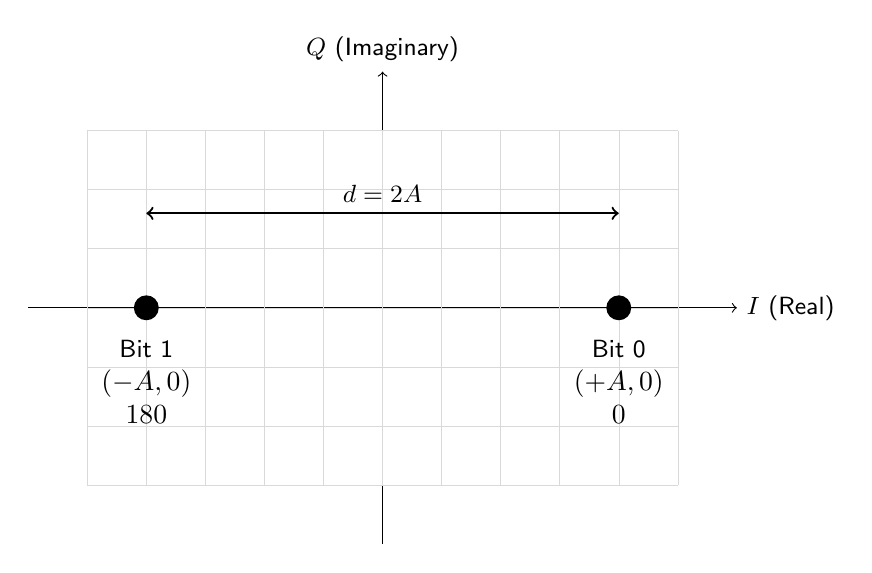
\begin{tikzpicture}[scale=1.5]
% Axes
\draw[->] (-3,0) -- (3,0) node[right] {\sffamily\small $I$ (Real)};
\draw[->] (0,-2) -- (0,2) node[above] {\sffamily\small $Q$ (Imaginary)};

% Grid
\draw[very thin,gray!30] (-2.5,-1.5) grid[step=0.5] (2.5,1.5);

% Constellation points
\fill[black] (-2,0) circle (3pt);
\fill[black] (2,0) circle (3pt);

% Labels
\node[below=8pt,align=center] at (-2,0) {\sffamily\small Bit 1\\$(-A, 0)$\\$180°$};
\node[below=8pt,align=center] at (2,0) {\sffamily\small Bit 0\\$(+A, 0)$\\$0°$};

% Distance annotation
\draw[<->,thick] (-2,0.8) -- (2,0.8) node[midway,above] {\sffamily\small $d = 2A$};
\end{tikzpicture}
\end{center}

This maximum Euclidean separation between symbols provides optimal noise immunity for binary modulation schemes.

\section{Modulation and Demodulation}

\subsection{Transmitter (Modulator)}

The BPSK modulator consists of three stages:

\begin{center}
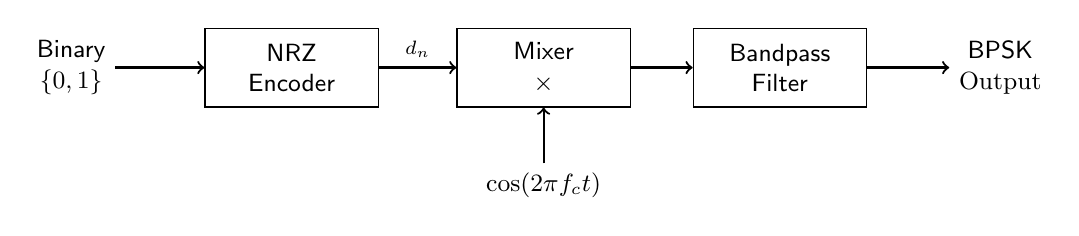
\begin{tikzpicture}[
  block/.style={rectangle, draw, minimum width=2.2cm, minimum height=1cm, font=\sffamily\small, align=center},
  node distance=2.2cm,
  font=\small
]
\node[align=center] (input) {\sffamily Binary\\$\{0, 1\}$};
\node[block, right of=input, node distance=2.8cm] (nrz) {NRZ\\Encoder};
\node[block, right of=nrz, node distance=3.2cm] (mult) {Mixer\\$\times$};
\node[block, right of=mult, node distance=3cm] (filter) {Bandpass\\Filter};
\node[align=center, right of=filter, node distance=2.8cm] (output) {\sffamily BPSK\\Output};

\node[below of=mult, node distance=1.5cm, font=\small] (carrier) {$\cos(2\pi f_c t)$};

\draw[->,thick] (input) -- (nrz);
\draw[->,thick] (nrz) -- node[above,font=\scriptsize] {$d_n$} (mult);
\draw[->,thick] (carrier) -- (mult);
\draw[->,thick] (mult) -- (filter);
\draw[->,thick] (filter) -- (output);
\end{tikzpicture}
\end{center}

\textbf{Process:}
\begin{enumerate}
\item \textbf{NRZ encoding:} Map bits to bipolar symbols
  \begin{itemize}
  \item Bit 0 $\rightarrow$ $d_n = +1$
  \item Bit 1 $\rightarrow$ $d_n = -1$
  \end{itemize}
\item \textbf{Multiply by carrier:} $s(t) = A \cdot d_n \cdot \cos(2\pi f_c t)$
\item \textbf{Pulse shaping:} Apply raised-cosine filter to:
  \begin{itemize}
  \item Limit occupied bandwidth
  \item Prevent intersymbol interference (ISI)
  \item Meet spectral mask requirements
  \end{itemize}
\end{enumerate}

\subsection{Receiver (Coherent Detector)}

\begin{center}
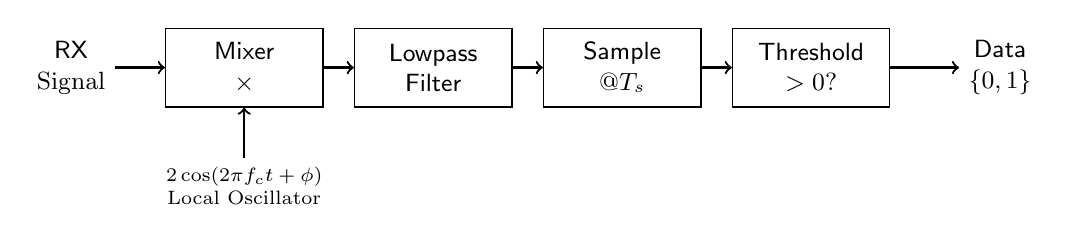
\begin{tikzpicture}[
  block/.style={rectangle, draw, minimum width=2cm, minimum height=1cm, font=\sffamily\small, align=center},
  node distance=2cm,
  font=\small
]
\node[align=center] (input) {\sffamily RX\\Signal};
\node[block, right of=input, node distance=2.2cm] (mult) {Mixer\\$\times$};
\node[block, right of=mult, node distance=2.4cm] (lpf) {Lowpass\\Filter};
\node[block, right of=lpf, node distance=2.4cm] (sample) {Sample\\$@T_s$};
\node[block, right of=sample, node distance=2.4cm] (thresh) {Threshold\\$>0?$};
\node[align=center, right of=thresh, node distance=2.4cm] (output) {\sffamily Data\\$\{0,1\}$};

\node[below of=mult, node distance=1.5cm, font=\scriptsize, align=center] (lo) {$2\cos(2\pi f_c t + \phi)$\\Local Oscillator};

\draw[->,thick] (input) -- (mult);
\draw[->,thick] (lo) -- (mult);
\draw[->,thick] (mult) -- (lpf);
\draw[->,thick] (lpf) -- (sample);
\draw[->,thick] (sample) -- (thresh);
\draw[->,thick] (thresh) -- (output);
\end{tikzpicture}
\end{center}

\begin{warningbox}
\textbf{Phase synchronization is critical.} The local oscillator must be exactly in phase with the transmitter carrier. A phase offset $\phi_e$ reduces detected signal by $\cos(\phi_e)$. At $\phi_e = 90°$, complete signal loss occurs.
\end{warningbox}

\textbf{Detection process:}

\begin{enumerate}
\item \textbf{Multiply by local carrier} (frequency $f_c$, phase $\phi = 0$):
\begin{equation}
r(t) = s(t) \cdot 2\cos(2\pi f_c t) = 2A d_n \cos^2(2\pi f_c t)
\end{equation}

\item \textbf{Apply trigonometric identity} $\cos^2(x) = \frac{1}{2}[1 + \cos(2x)]$:
\begin{equation}
r(t) = A d_n [1 + \cos(4\pi f_c t)]
\end{equation}

\item \textbf{Lowpass filter} removes $2f_c$ component, leaving baseband:
\begin{equation}
y(t) = A d_n
\end{equation}

\item \textbf{Sample at bit period} $T_b$: $y_n = A d_n + n(t)$ where $n(t)$ is AWGN

\item \textbf{Threshold decision:}
\begin{equation}
\hat{d}_n = \begin{cases}
+1 & \text{if } y_n > 0 \quad \text{(decode as bit 0)} \\
-1 & \text{if } y_n < 0 \quad \text{(decode as bit 1)}
\end{cases}
\end{equation}
\end{enumerate}

\section{Carrier Recovery}

The receiver must generate a local oscillator \textbf{exactly in phase} with the transmitter carrier. This is the primary challenge in coherent BPSK detection.

\subsection{Problem: Phase Ambiguity}

A phase offset $\phi_e$ between transmitter and receiver carriers causes:
\begin{equation}
y(t) = A d_n \cos(\phi_e) + n(t)
\end{equation}

\textbf{Effects:}
\begin{itemize}
\item $\phi_e = 0°$: Full signal strength (optimal)
\item $\phi_e = 45°$: Signal reduced by 3~dB
\item $\phi_e = 90°$: Complete signal loss
\item $\phi_e = 180°$: Inverted data (all bits flipped)
\end{itemize}

\subsection{Carrier Recovery Techniques}

\subsubsection{1. Pilot Tone}
\begin{itemize}
\item[\checkmark] Simple implementation
\item[\checkmark] Accurate phase reference
\item[\texttimes] Wastes power (typically 10--20\% of total)
\item[\texttimes] Reduces data throughput
\end{itemize}

\subsubsection{2. Costas Loop}
PLL-based carrier recovery using I/Q demodulation:
\begin{itemize}
\item[\checkmark] No pilot tone required
\item[\checkmark] Optimal for BPSK and QPSK
\item[\texttimes] Complex analog circuitry
\item[\texttimes] Acquisition time required
\end{itemize}

\subsubsection{3. Squaring Loop}
Exploits $d_n^2 = 1$ to remove data modulation:
\begin{equation}
[d_n \cos(2\pi f_c t)]^2 = \frac{1}{2}[1 + \cos(4\pi f_c t)]
\end{equation}
PLL locks to $2f_c$, then divides by 2 to recover $f_c$.
\begin{itemize}
\item[\checkmark] Completely removes data modulation
\item[\checkmark] Robust in low SNR
\item[\texttimes] $180°$ phase ambiguity (requires differential encoding)
\end{itemize}

\subsection{Differential BPSK (DBPSK)}

\textbf{Principle:} Encode data in \textbf{phase transitions}, not absolute phase.

\textbf{Encoding rule:}
\begin{equation}
\phi_n = \phi_{n-1} + \Delta\phi_n \quad\text{where}\quad \Delta\phi_n = \begin{cases}
0° & \text{if bit = 0} \\
180° & \text{if bit = 1}
\end{cases}
\end{equation}

\textbf{Decoding:} Compare consecutive symbols:
\begin{equation}
\hat{b}_n = \begin{cases}
0 & \text{if } \mathrm{sgn}(y_n) = \mathrm{sgn}(y_{n-1}) \\
1 & \text{if } \mathrm{sgn}(y_n) \neq \mathrm{sgn}(y_{n-1})
\end{cases}
\end{equation}

\textbf{Trade-off:}
\begin{itemize}
\item[\checkmark] No carrier recovery needed
\item[\checkmark] Simpler receiver
\item[\texttimes] Approximately 3~dB performance penalty
\item[\texttimes] Error propagation (single error affects two bits)
\end{itemize}

\section{Bit Error Rate (BER) Performance}

\subsection{Coherent BPSK in AWGN Channel}

For ideal coherent detection with perfect synchronization:
\begin{equation}
\mathrm{BER} = Q\left(\sqrt{\frac{2E_b}{N_0}}\right) = \frac{1}{2}\mathrm{erfc}\left(\sqrt{\frac{E_b}{N_0}}\right)
\end{equation}
where:
\begin{itemize}
\item $E_b = \frac{A^2 T_b}{2}$ = energy per bit (joules)
\item $N_0$ = noise power spectral density (W/Hz)
\item $Q(x) = \frac{1}{\sqrt{2\pi}}\int_x^\infty e^{-t^2/2}\,dt$ (Gaussian Q-function)
\end{itemize}

\textbf{Performance benchmarks:}

\begin{center}
\begin{tabular}{@{}lrl@{}}
\toprule
$E_b/N_0$ (dB) & \multicolumn{1}{c}{BER} & Practical Meaning \\
\midrule
0~dB & $7.9 \times 10^{-2}$ & 1 error in 13 bits \\
5~dB & $9.7 \times 10^{-4}$ & 1 error in 1,000 bits \\
10~dB & $3.9 \times 10^{-6}$ & 1 error in 250,000 bits \\
15~dB & $6.9 \times 10^{-10}$ & 1 error in 1.4 billion bits \\
\bottomrule
\end{tabular}
\end{center}

\subsection{Comparison: BPSK vs OOK}

At the same $E_b/N_0 = 10$~dB:

\begin{center}
\begin{tabular}{@{}lrr@{}}
\toprule
Modulation Scheme & BER & Performance Ratio \\
\midrule
OOK (non-coherent) & $4.0 \times 10^{-3}$ & Baseline \\
\textbf{BPSK (coherent)} & $\mathbf{3.9 \times 10^{-6}}$ & \textbf{1000$\times$ better} \\
\bottomrule
\end{tabular}
\end{center}

\begin{keyconcept}
\textbf{Why is BPSK 3~dB better than OOK?}

\begin{enumerate}
\item \textbf{Full signal space utilization:} BPSK uses $\pm A$ (both polarities), while OOK uses $\{0, A\}$ (one polarity). This doubles the Euclidean distance between symbols.

\item \textbf{Coherent detection:} Correlating with a known carrier phase is the optimal detection strategy (maximum likelihood).

\item \textbf{Constant envelope:} Energy is transmitted continuously, not just during ``on'' bits.
\end{enumerate}
\end{keyconcept}

\subsection{Differential BPSK Performance}

DBPSK trades synchronization complexity for performance:
\begin{equation}
\mathrm{BER}_{\mathrm{DBPSK}} \approx \frac{1}{2}e^{-E_b/N_0}
\end{equation}

At $E_b/N_0 = 10$~dB: BER $\approx 5 \times 10^{-6}$ (approximately 1.3~dB penalty versus coherent BPSK).

\section{Bandwidth Efficiency}

The occupied bandwidth (99\% power) for rectangular pulses is:
\begin{equation}
B \approx \frac{1}{T_b} = R_b
\end{equation}
where $R_b$ is the bit rate (bps) and $T_b$ is the bit period (seconds).

With \textbf{raised-cosine pulse shaping} (roll-off factor $\alpha$):
\begin{equation}
B = R_b(1 + \alpha)
\end{equation}

\textbf{Typical value:} $\alpha = 0.35$ gives $B = 1.35 R_b$

\textbf{Spectral efficiency:}
\begin{equation}
\eta = \frac{R_b}{B} = \frac{1}{1+\alpha} \approx 0.74\ \text{bps/Hz}
\end{equation}

\begin{calloutbox}{Example: 1~Mbps BPSK System}
\begin{itemize}
\item Data rate: $R_b = 1$~Mbps
\item Roll-off: $\alpha = 0.35$
\item Required bandwidth: $B = 1 \times (1 + 0.35) = 1.35$~MHz
\item Spectral efficiency: $\eta = 1/1.35 = 0.74$~bps/Hz
\end{itemize}
\end{calloutbox}

\section{Practical Implementations}

\subsection{IEEE 802.15.4 (Zigbee)}

Low-rate wireless personal area networks (868/915~MHz bands):
\begin{itemize}
\item \textbf{Modulation:} BPSK with Direct-Sequence Spread Spectrum (DSSS)
\item \textbf{Chip rate:} 300~kcps (868~MHz), 600~kcps (915~MHz)
\item \textbf{Data rate:} 20~kbps (868~MHz), 40~kbps (915~MHz)
\item \textbf{Spreading gain:} 15:1 to 20:1 (improves interference rejection)
\end{itemize}

\subsection{Satellite Telemetry}

Deep-space missions (Voyager, Mars rovers) use BPSK for maximum power efficiency:
\begin{itemize}
\item \textbf{Modulation:} BPSK or QPSK
\item \textbf{Coding:} Concatenated (Convolutional + Reed-Solomon)
\item \textbf{Data rate:} 10~bps to 10~kbps (extreme path loss)
\item \textbf{Rationale:} Every dB matters at interplanetary distances
\end{itemize}

\begin{calloutbox}[colback=black!5!white,colframe=black]{Example: Voyager 1 at 24 Billion km}
\begin{tabular}{@{}ll@{}}
TX power & 23~W \\
TX antenna gain & 48~dBi (3.7~m dish) \\
RX antenna & 70~m Deep Space Network dish (74~dBi) \\
Free-space path loss & 310~dB \\
Received power & $-196$~dBm \\
Link budget & Barely positive with FEC \\
Achieved BER & $\sim 10^{-5}$ \\
\end{tabular}
\end{calloutbox}

\subsection{RFID Backscatter}

Passive RFID tags use backscatter modulation (effectively BPSK):
\begin{itemize}
\item \textbf{Mechanism:} Tag switches antenna impedance (reflection vs absorption)
\item \textbf{Binary encoding:} Reflection = bit 0, absorption = bit 1
\item \textbf{Data rate:} 40--640~kbps (EPC Gen2 standard)
\item \textbf{Power source:} Harvested from reader's carrier
\end{itemize}

\section{Advantages and Disadvantages}

\subsection*{Advantages}

\begin{enumerate}
\item \textbf{Optimal binary modulation:} Best BER performance for 1 bit/symbol (3~dB better than OOK)
\item \textbf{Constant envelope:} Compatible with nonlinear amplifiers (no AM-PM distortion)
\item \textbf{Simple constellation:} Two points simplify visualization and analysis
\item \textbf{Foundation for higher PSK:} Concepts extend naturally to QPSK, 8PSK, etc.
\end{enumerate}

\subsection*{Disadvantages}

\begin{enumerate}
\item \textbf{Carrier synchronization required:} Costas loop or squaring loop adds complexity
\item \textbf{DBPSK penalty:} Avoiding synchronization costs 3~dB in performance
\item \textbf{Low spectral efficiency:} 1 bit/symbol = maximum 1~bps/Hz
\item \textbf{Outperformed at high SNR:} QPSK, 16-QAM more efficient when SNR permits
\end{enumerate}

\section{Transition to Higher-Order Modulation}

BPSK uses only the I-axis (real axis) with two constellation points.

\textbf{Natural extension:} Utilize \textbf{both I and Q axes} to create QPSK:

\begin{center}
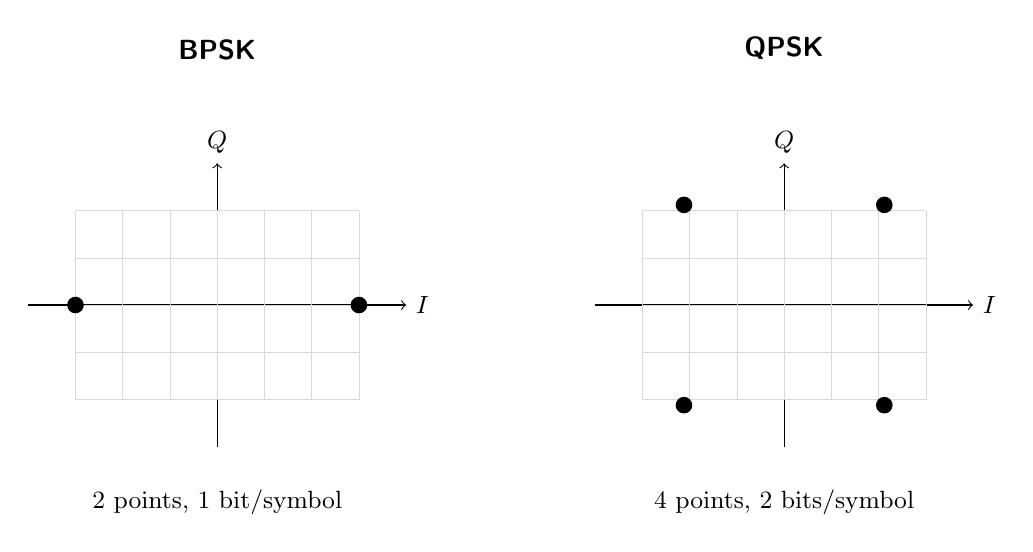
\begin{tikzpicture}[scale=1.2]
% BPSK
\begin{scope}[shift={(0,0)}]
\node[above,font=\sffamily\bfseries] at (0,2.5) {BPSK};
\draw[->] (-2,0) -- (2,0) node[right,font=\sffamily\small] {$I$};
\draw[->] (0,-1.5) -- (0,1.5) node[above,font=\sffamily\small] {$Q$};
\draw[very thin,gray!30] (-1.5,-1) grid[step=0.5] (1.5,1);
\fill[black] (-1.5,0) circle (2.5pt);
\fill[black] (1.5,0) circle (2.5pt);
\node[below=12pt,font=\small] at (0,-1.5) {2 points, 1 bit/symbol};
\end{scope}

% QPSK
\begin{scope}[shift={(6,0)}]
\node[above,font=\sffamily\bfseries] at (0,2.5) {QPSK};
\draw[->] (-2,0) -- (2,0) node[right,font=\sffamily\small] {$I$};
\draw[->] (0,-1.5) -- (0,1.5) node[above,font=\sffamily\small] {$Q$};
\draw[very thin,gray!30] (-1.5,-1) grid[step=0.5] (1.5,1);
\fill[black] (1.06,1.06) circle (2.5pt);
\fill[black] (-1.06,1.06) circle (2.5pt);
\fill[black] (-1.06,-1.06) circle (2.5pt);
\fill[black] (1.06,-1.06) circle (2.5pt);
\node[below=12pt,font=\small] at (0,-1.5) {4 points, 2 bits/symbol};
\end{scope}
\end{tikzpicture}
\end{center}

\textbf{QPSK} = Two independent BPSK channels (I and Q) operating in parallel, doubling spectral efficiency to $\sim$2~bps/Hz.

\section{Worked Example: Satellite Link Budget}

\textbf{Scenario:} Geostationary satellite downlink to 1~m ground station

\subsection*{Given Parameters}

\begin{tabular}{@{}ll@{}}
TX power & $P_t = 10$~W = 40~dBm \\
TX antenna gain & $G_t = 30$~dBi \\
Distance & $d = 36{,}000$~km (GEO orbit) \\
Frequency & $f = 12$~GHz (Ku-band) \\
RX antenna gain & $G_r = 40$~dBi (1~m dish) \\
System noise temp & $T_s = 150$~K \\
Bandwidth & $B = 1$~MHz \\
Required BER & $10^{-6}$ \\
\end{tabular}

\subsection*{Step 1: Free-Space Path Loss}

\begin{equation}
\mathrm{FSPL\,[dB]} = 20\log_{10}(d_{\text{km}}) + 20\log_{10}(f_{\text{MHz}}) + 32.45
\end{equation}
\begin{equation}
\mathrm{FSPL} = 20\log_{10}(36{,}000) + 20\log_{10}(12{,}000) + 32.45 = 205.5~\text{dB}
\end{equation}

\subsection*{Step 2: Received Signal Power}

\begin{equation}
P_r = P_t + G_t + G_r - \mathrm{FSPL}
\end{equation}
\begin{equation}
P_r = 40 + 30 + 40 - 205.5 = -95.5~\text{dBm}
\end{equation}

\subsection*{Step 3: Noise Power}

\begin{equation}
N = kT_sB = (1.38 \times 10^{-23})(150)(10^6) = 2.07 \times 10^{-15}~\text{W}
\end{equation}
\begin{equation}
N = 10\log_{10}(2.07 \times 10^{-15} / 10^{-3}) = -117~\text{dBm}
\end{equation}

\subsection*{Step 4: Signal-to-Noise Ratio}

\begin{equation}
\mathrm{SNR} = P_r - N = -95.5 - (-117) = 21.5~\text{dB}
\end{equation}

\subsection*{Step 5: Energy-per-Bit to Noise Ratio}

Assuming data rate $R_b = 500$~kbps:
\begin{equation}
\frac{E_b}{N_0} = \mathrm{SNR} + 10\log_{10}\left(\frac{B}{R_b}\right)
\end{equation}
\begin{equation}
\frac{E_b}{N_0} = 21.5 + 10\log_{10}\left(\frac{1{,}000{,}000}{500{,}000}\right) = 21.5 + 3.0 = 24.5~\text{dB}
\end{equation}

\subsection*{Step 6: Link Margin Calculation}

\begin{itemize}
\item \textbf{Required $E_b/N_0$ for BER $= 10^{-6}$:} 10.5~dB
\item \textbf{Available $E_b/N_0$:} 24.5~dB
\item \textbf{Link margin:} $24.5 - 10.5 = 14.0$~dB
\end{itemize}

\begin{calloutbox}[colback=black!8!white,colframe=black]{Link Budget Summary}
\textbf{Result: Link closes with 14~dB margin}

This comfortable margin accommodates:
\begin{itemize}
\item Rain fade ($\sim$5--8~dB at Ku-band)
\item Implementation losses ($\sim$2--3~dB)
\item Pointing errors ($\sim$1--2~dB)
\item Aging and component degradation
\end{itemize}

\textbf{Conclusion:} Link is viable for reliable 500~kbps BPSK transmission.
\end{calloutbox}

\section{Summary}

\begin{center}
\begin{tabular}{@{}ll@{}}
\toprule
\textbf{Parameter} & \textbf{Value} \\
\midrule
Bits per symbol & 1 \\
Constellation points & 2 ($0°$, $180°$) \\
Spectral efficiency & $\sim$0.7--1.0~bps/Hz \\
BER @ 10~dB $E_b/N_0$ & $3.9 \times 10^{-6}$ \\
Carrier recovery & Required (Costas/squaring loop) \\
Implementation & Moderate complexity \\
Best application & Power-limited channels \\
Typical uses & Satellite, deep-space, RFID \\
\bottomrule
\end{tabular}
\end{center}

\section{Further Reading}

\begin{itemize}
\item \textbf{Chapter 5:} On-Off Keying (OOK)---simpler but inferior performance
\item \textbf{Chapter 6:} Frequency-Shift Keying (FSK)---alternative binary scheme
\item \textbf{Chapter 7:} Quadrature Phase-Shift Keying (QPSK)---2 bits/symbol extension
\item \textbf{Chapter 12:} Constellation Diagrams---visualization techniques
\item \textbf{Chapter 13:} IQ Representation---complex baseband mathematics
\item \textbf{Chapter 18:} Bit Error Rate Analysis---performance measurement
\item \textbf{Chapter 22:} Forward Error Correction---coding for BER improvement
\item \textbf{Chapter 25:} Carrier Recovery Techniques---synchronization methods
\end{itemize}
